\documentclass[11pt]{article}
\usepackage[utf8]{inputenc}
\usepackage[dvips]{graphicx}
\usepackage{fancybox}
\usepackage{verbatim}
\usepackage{array}
\usepackage{latexsym}
\usepackage{alltt}
\usepackage{hyperref}
\usepackage{textcomp}
\usepackage{color}
\usepackage{amsmath}
\usepackage{amsfonts}
\usepackage{rotating}
\usepackage{tikz}
%\usepackage{fitch}  % to use fitch
\usepackage{float}
\usepackage[hmargin=3cm,vmargin=5.0cm]{geometry}
\usepackage{graphicx}
\graphicspath{ {./} }
%\topmargin=0cm
\topmargin=-2cm
\addtolength{\textheight}{6.5cm}
\addtolength{\textwidth}{2.0cm}
%\setlength{\leftmargin}{-5cm}
\setlength{\oddsidemargin}{0.0cm}
\setlength{\evensidemargin}{0.0cm}

\author{
  \textbf{Full Name:} Ahmet Eren Çolak\\
  \textbf{ID Number:} 2587921
}

\title{\textbf{CENG 435 - Data Communications and Networking\\
Take Home Exam 4 Solutions}}

\makeatletter
\renewcommand*\env@matrix[1][*\c@MaxMatrixCols c]{%
  \hskip -\arraycolsep
  \let\@ifnextchar\new@ifnextchar
  \array{#1}}
\makeatother



\begin{document}
	\maketitle

	\section*{Screenshots}

	\begin{figure}[h]
		\centering
		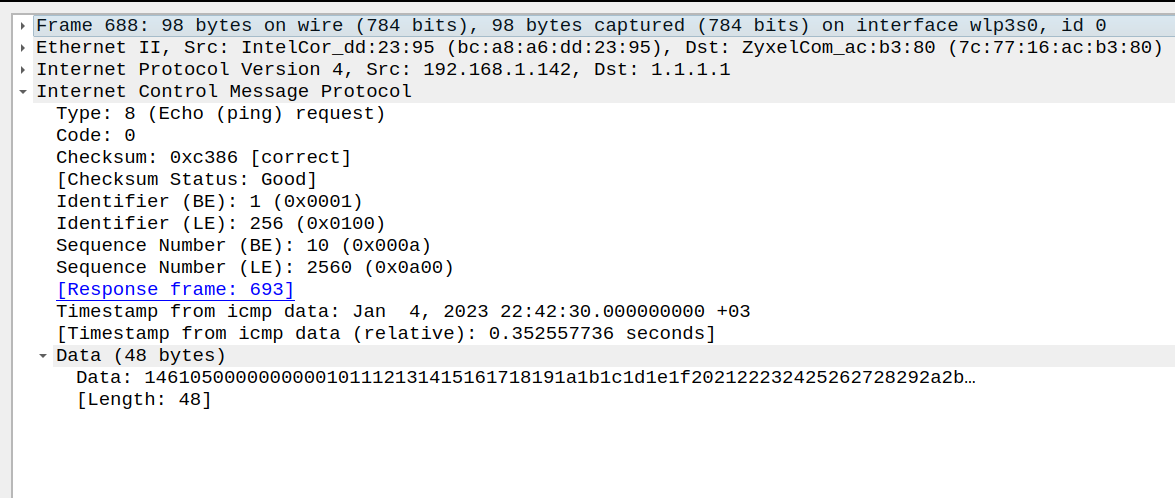
\includegraphics[scale=0.4]{request}
		\caption{Echo request message}
	\end{figure}
	
	\begin{figure}[h]
		\centering
		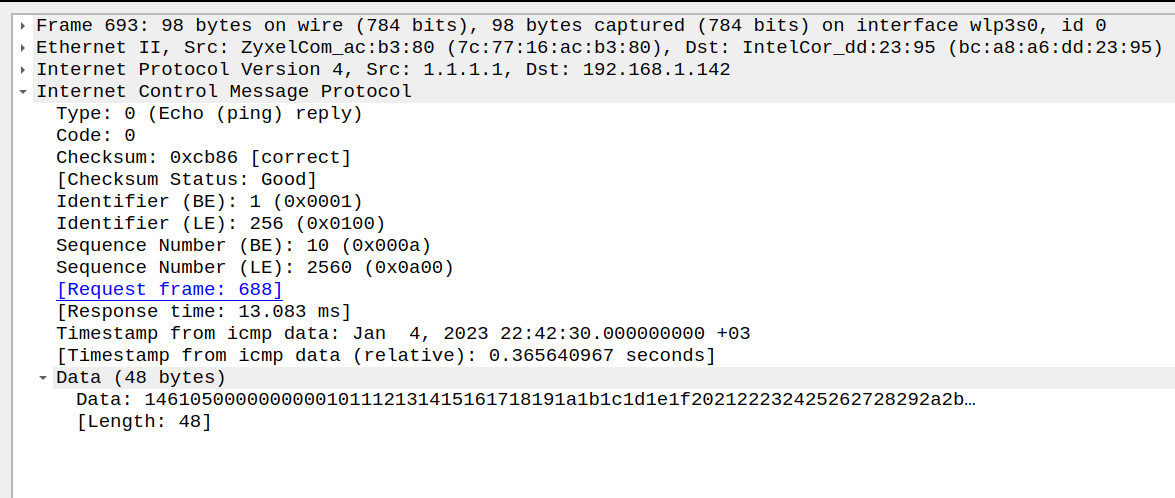
\includegraphics[scale=0.4]{response}
		\caption{Echo response message}
	\end{figure}
	
	\begin{figure}[h]
		\centering
		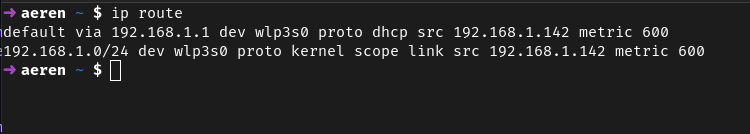
\includegraphics[scale=0.5]{iproute}
		\caption{IP route table}
	\end{figure}
	
	
	
	\break

	\section*{Q. 1}
	Source IP addresses of echo request messages are 192.168.1.142 which is my computer's IPv4 address. 
	Destination addresses of echo request messages are 192.168.1.1 which is my router's IPv4 address. 
	In echo response messages destination and source addresses are the opposite.

	\section*{Q. 2}
	There is no port number information in ICMP packets because ICMP protocol provides only host-to-host
	communication. Therefore there is no need for a port number information to match processes.
	
	\section*{Q. 3}
	\subsection*{a.} 
	Type field represents the type of the message. 
	Types of packets I captured are either echo request messages or echo response messages.
	
	\subsection*{b.}
	Code field provides additional information about the type of the message.

	\subsection*{c.}
	Value of 0 in type field represents \emph{echo response} messages and value of 8 in type field
	represents \emph{echo request} messages. Only value of code field for both echo request and response messages is 0 which does not
	provide any additional information about these type of messages.

	\section*{Q. 4}
	In total 64 bytes were sent. First byte is for the type field and second byte is for the code field.
	Following 2 bytes are for the checksum value to check the correctness of the package.
	Next 2 bytes are for identifier value and the following 2 bytes of identifier value are for sequence number.
	Identifier and sequence number field help with matching echo request and response messages.
	Next 8 bytes are for the timestamp value. Rest 48 bytes are reserved for data field which is not specified for echo request and response messages.

	\section*{Q. 5}
	Rule for default which routes to my router should be deleted. When this rule is deleted no packages will be able to reach router.
	Therefore no packages will be routed to correct hosts.
	
	\section*{Q. 6}
	\subsection*{a.}
	Ethernet address of my device is \emph{bc:a8:a6:dd:23:95}.
	\subsection*{b.}
	Destination Ethernet address is \emph{7c:77:16:ac:b3:80}. It is the Ethernet address of my router.
	\subsection*{c.}
	I encountered 3 values. These are IPv4, IPv6 and ARP. Since my router supports IPv6 protocol some ICMP messages are sent with IPv6.
	These ICMP messages which uses IPv6 are for \emph{router advertisement} messages which has type values of 134. ARP messages are sent because my router
	broadcasted an ARP message to match my devices IPv4 address with its Ethernet address.
\end{document}